\subsection{Field data}
Time-series data for field data from \textit{ORIENT NY} monitoring station; the data is collected at intervals of 6mins, with no data available represented by $NaN$.

As represented in Fig.\ref{fig:time_series_ny_temp}, the temperature shows a seasonal pattern at a frequency of 6-8 months, representing the gap between summer and winter seasons. Other parameters pH, dissolved oxygen, specific conductance and salinity also
follows a similar pattern with frequency around 6-months.


\begin{figure}[H]
    \hspace*{4cm}\subfloat[Temperature]{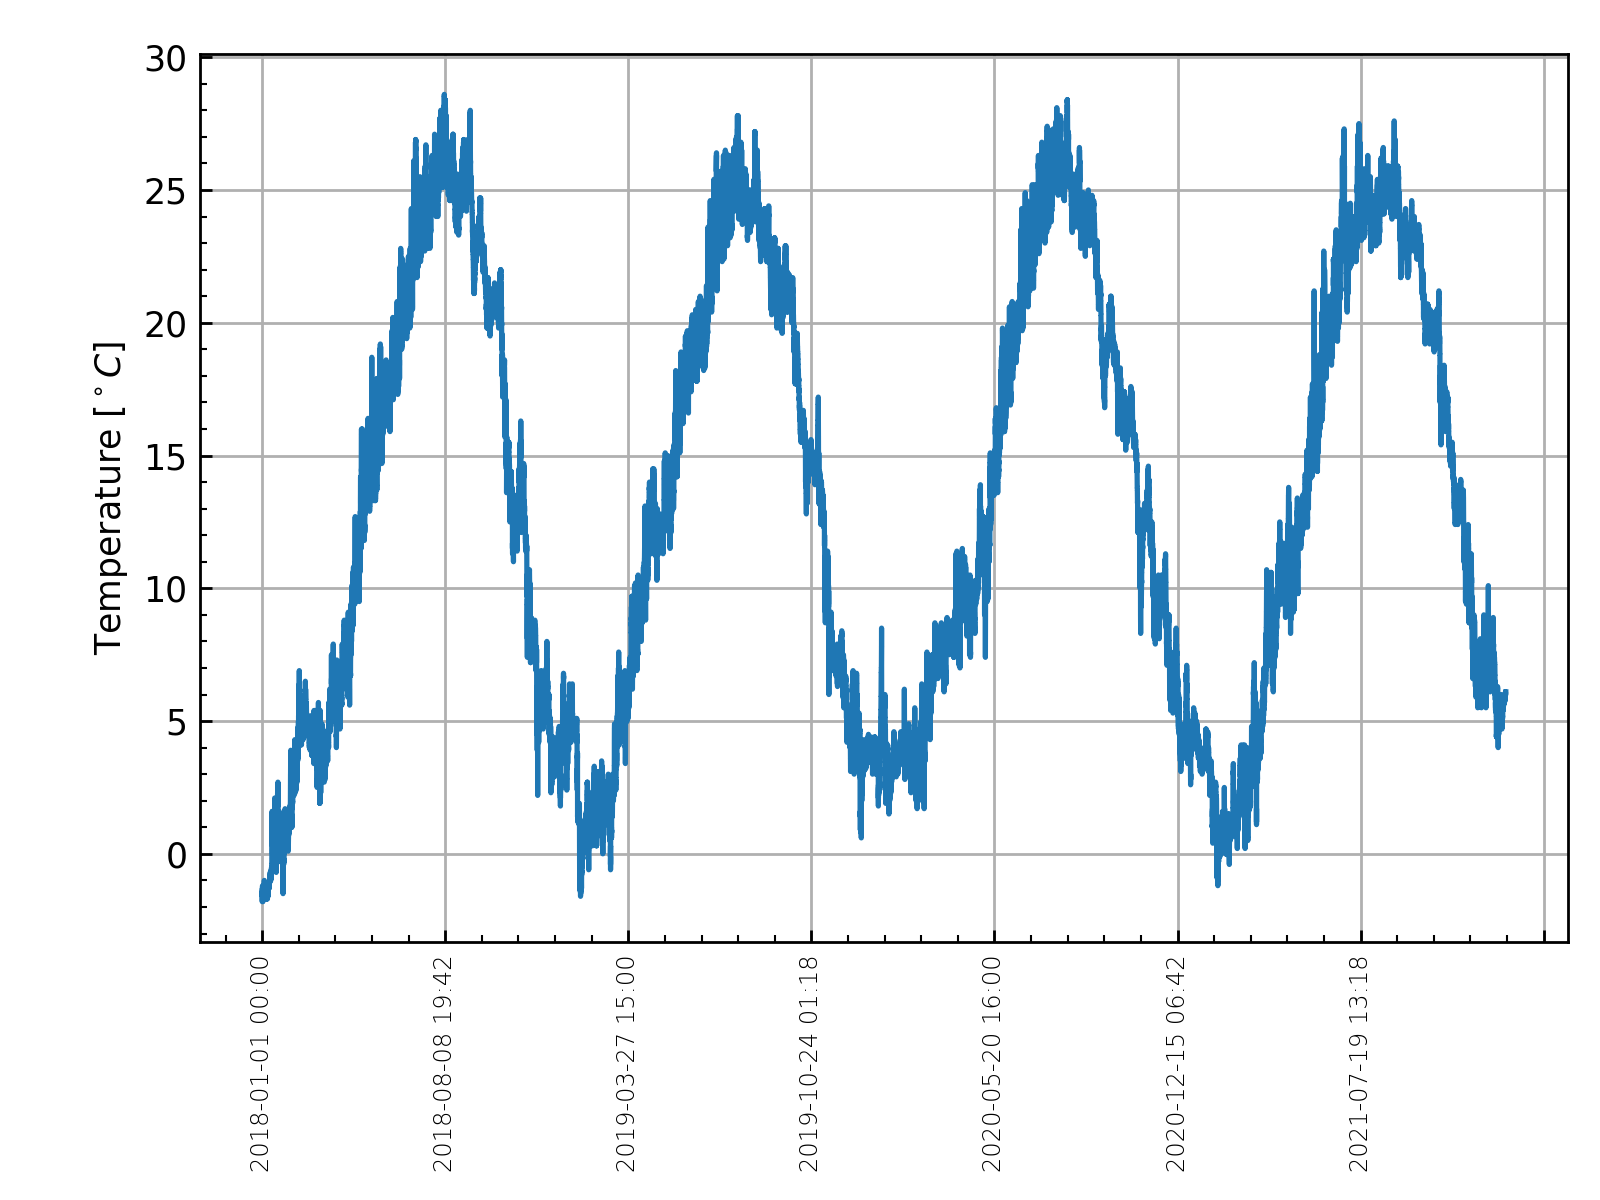
\includegraphics[scale=0.5]{figs/plots/temperature.png}\label{fig:time_series_ny_temp}} \\
    \subfloat[pH]{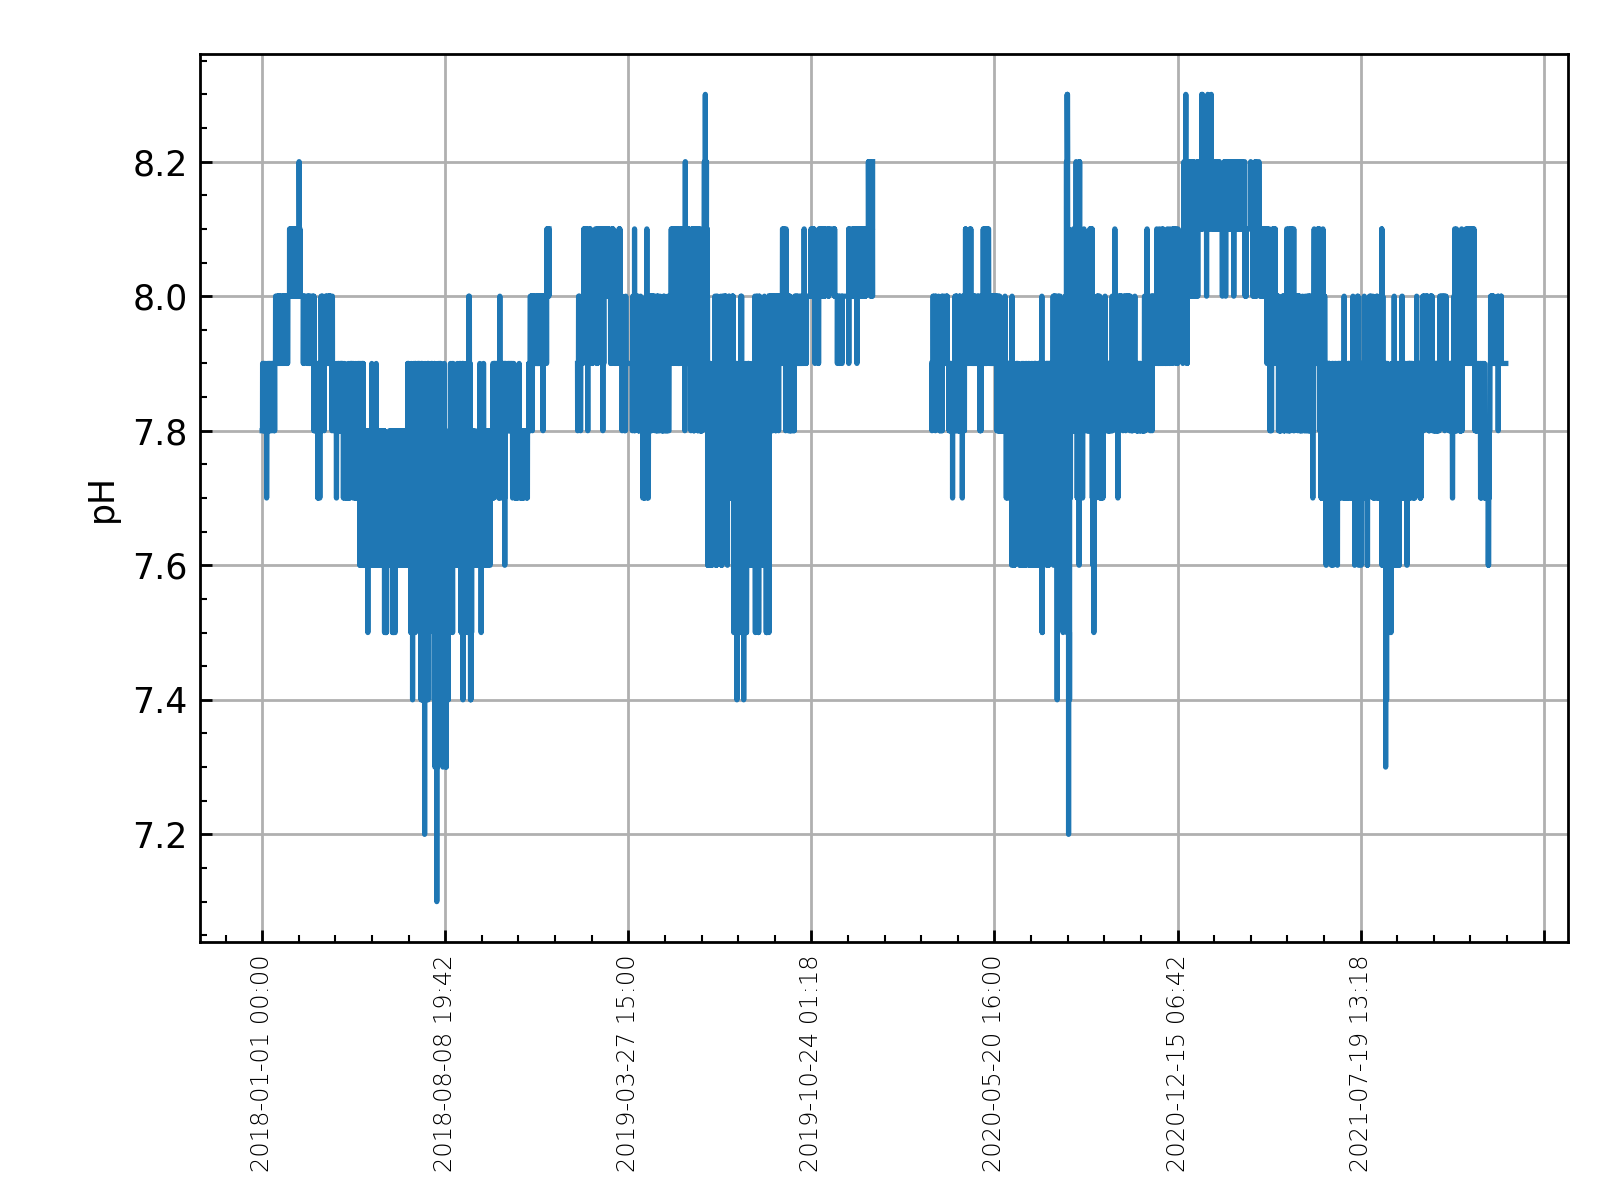
\includegraphics[scale=0.5]{figs/plots/pH.png}}
    \quad
    \subfloat[Dissolved oxygen(mg/L)]{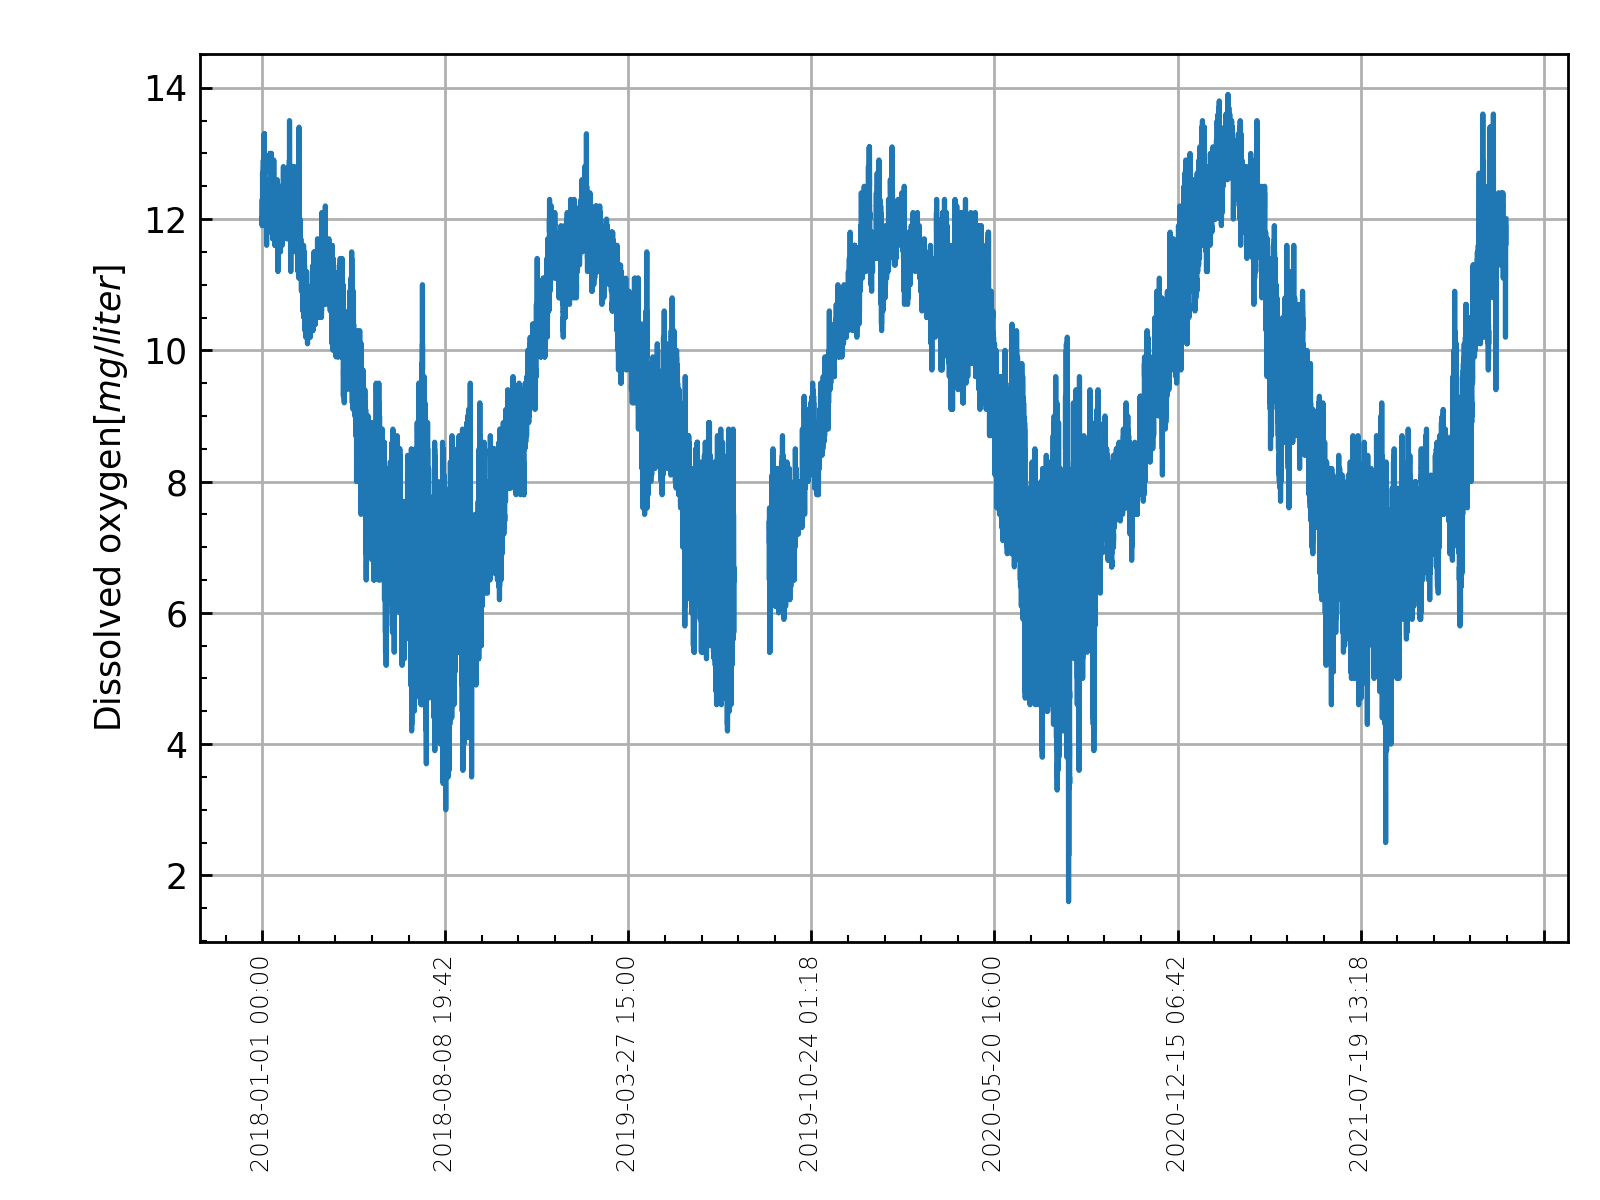
\includegraphics[scale=0.5]{figs/plots/do.png}\label{fig:time_series_ny_do}}
    \hfill
    \subfloat[Specific conductance($\mu S/cm$)]{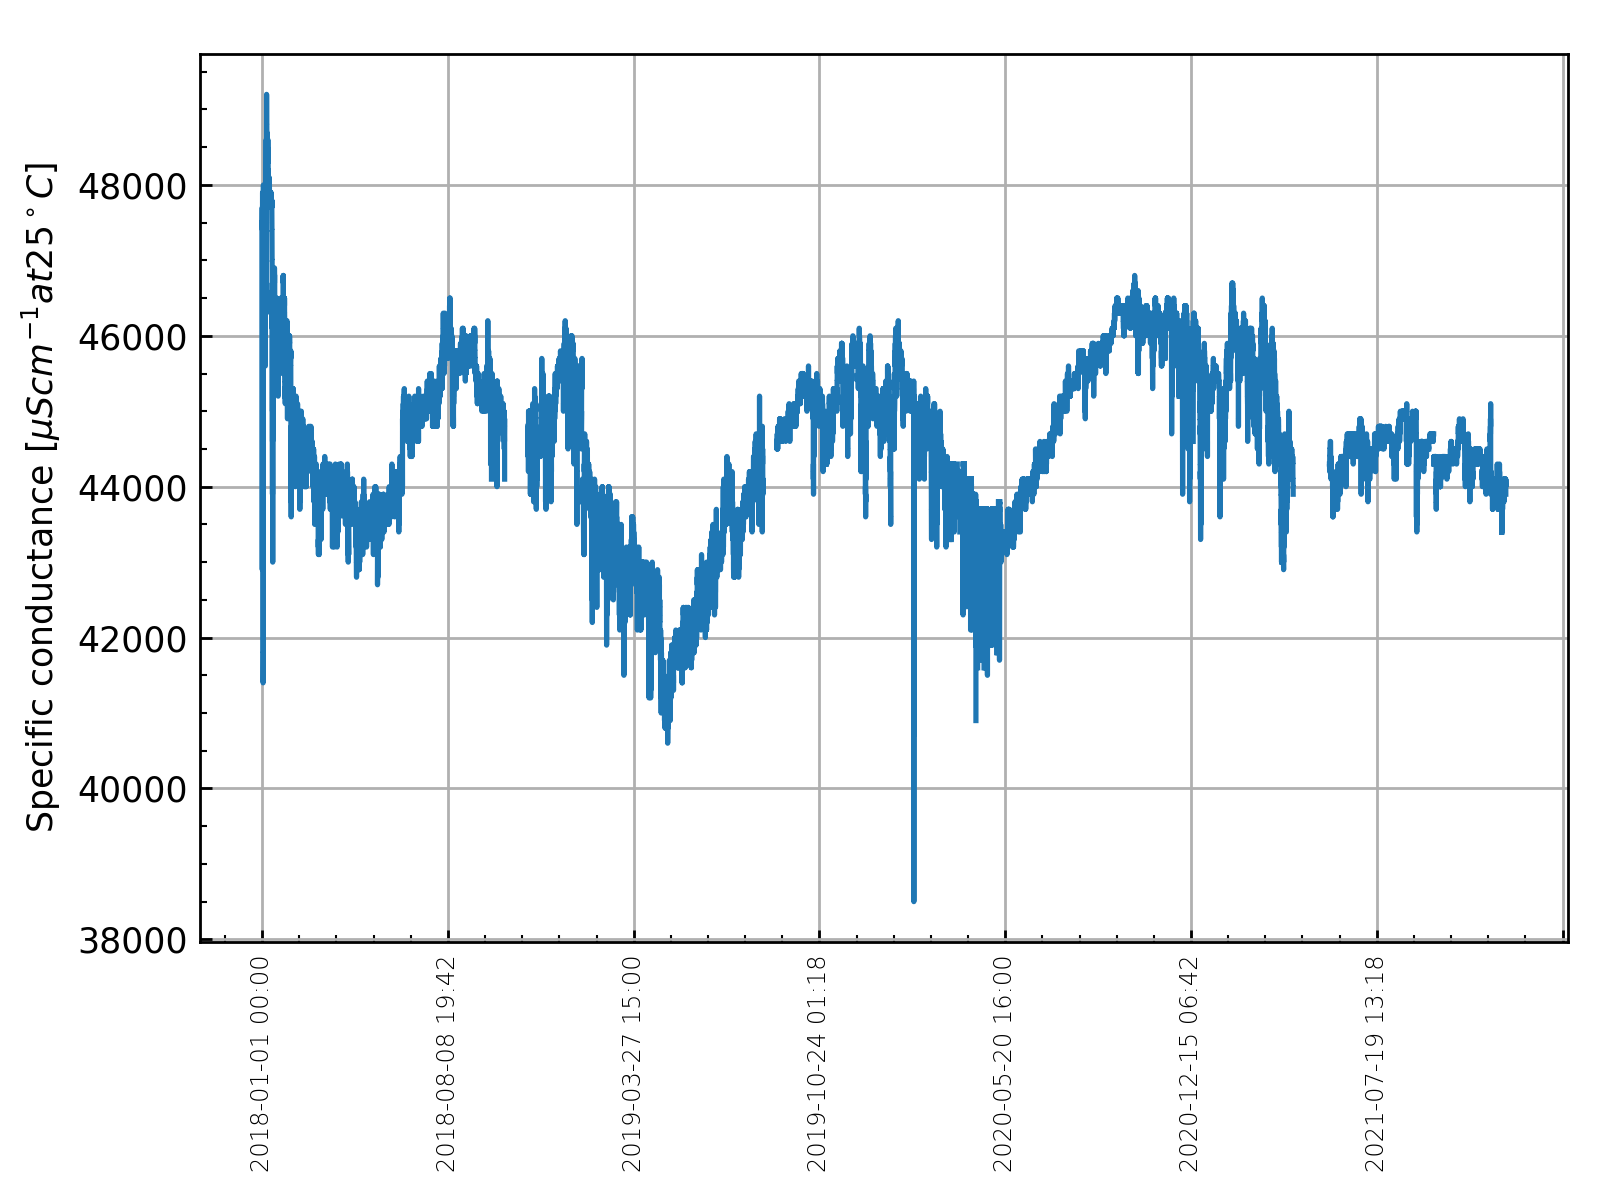
\includegraphics[scale=0.5]{figs/plots/conductance.png}}
    \quad
    \subfloat[Salinity($psu$)]{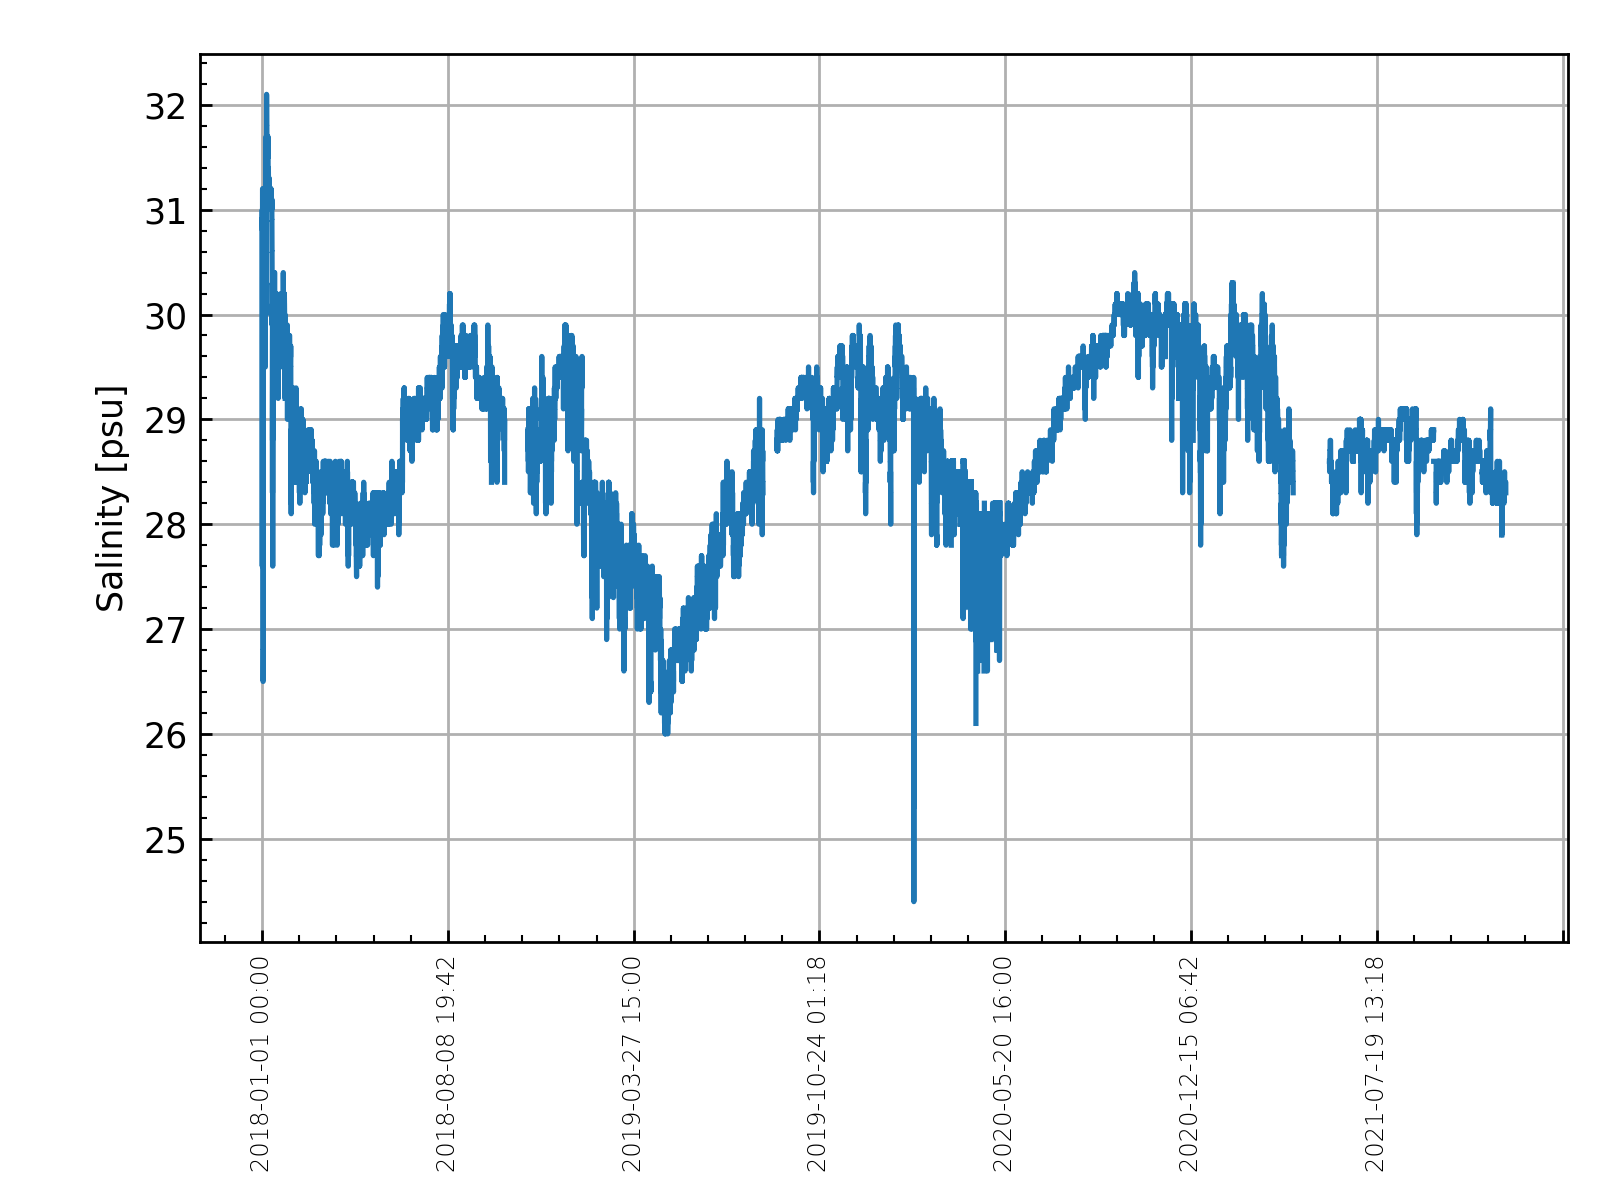
\includegraphics[scale=0.5]{figs/plots/salinity.png}}
    \caption{Orient Harbour New York, US}
\end{figure}

\paragraph{Correlation with dissolved oxygen}
By using our field data we can compute correlations matrices to solidfy our understanding of correlations between dissolved oxygen and pH, dissolved oxygen and specific conductance et al.

Through these correlation matrices we can verify that our parameters have a positive correlation with the concentration of dissolved oxygen.

\begin{figure}[H]
    \subfloat[Dissolved oxygen and salinity]{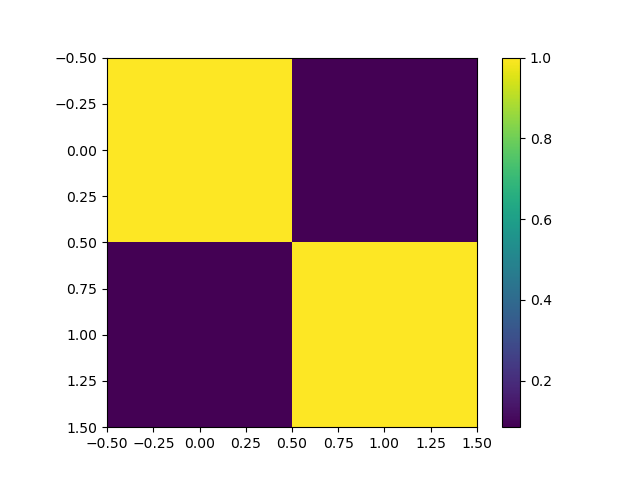
\includegraphics[scale=0.5]{figs/plots/do_vs_salinity.png}}
    \quad
    \subfloat[Dissolved oxygen and temperature]{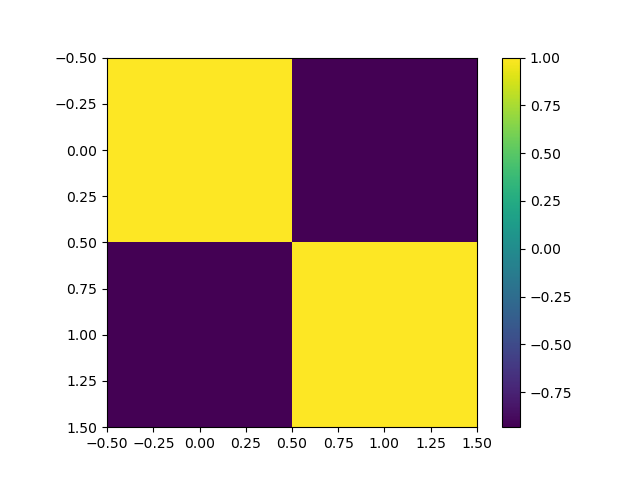
\includegraphics[scale=0.5]{figs/plots/do_vs_temp.png}}
    \hfill
    \subfloat[Dissolved oxygen and specific conductance]{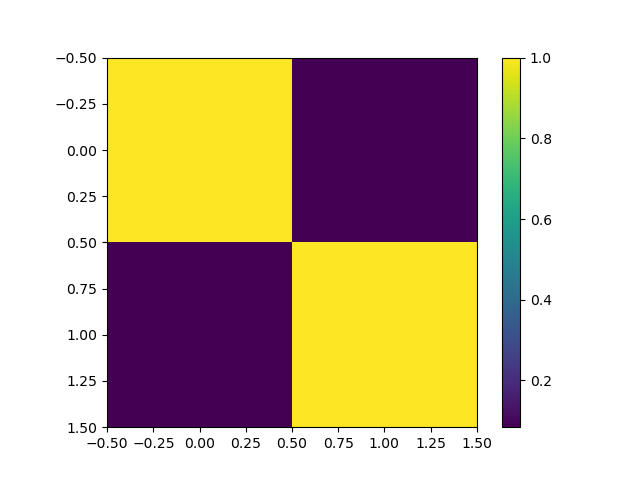
\includegraphics[scale=0.5]{figs/plots/do_vs_conductance.png}}
    \quad
    \subfloat[Dissolved oxygen and pH]{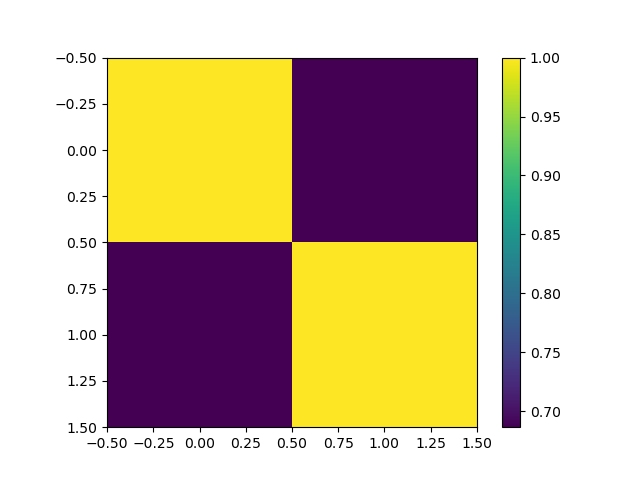
\includegraphics[scale=0.5]{figs/plots/do_vs_pH.png}}
    \caption{Correlation matrics with dissolved oxygen}
\end{figure}



\subsection{AQUA-MODIS data}
    Fig.15 represents the time-series data from the spatially averged AQUA-MODIS dataset for SST and Chlorophyll-A for our geofenced location of \textit{ORIENT NY}

\begin{figure}[H]
    \subfloat[SST($11\mu m$; $^\circ C$)]{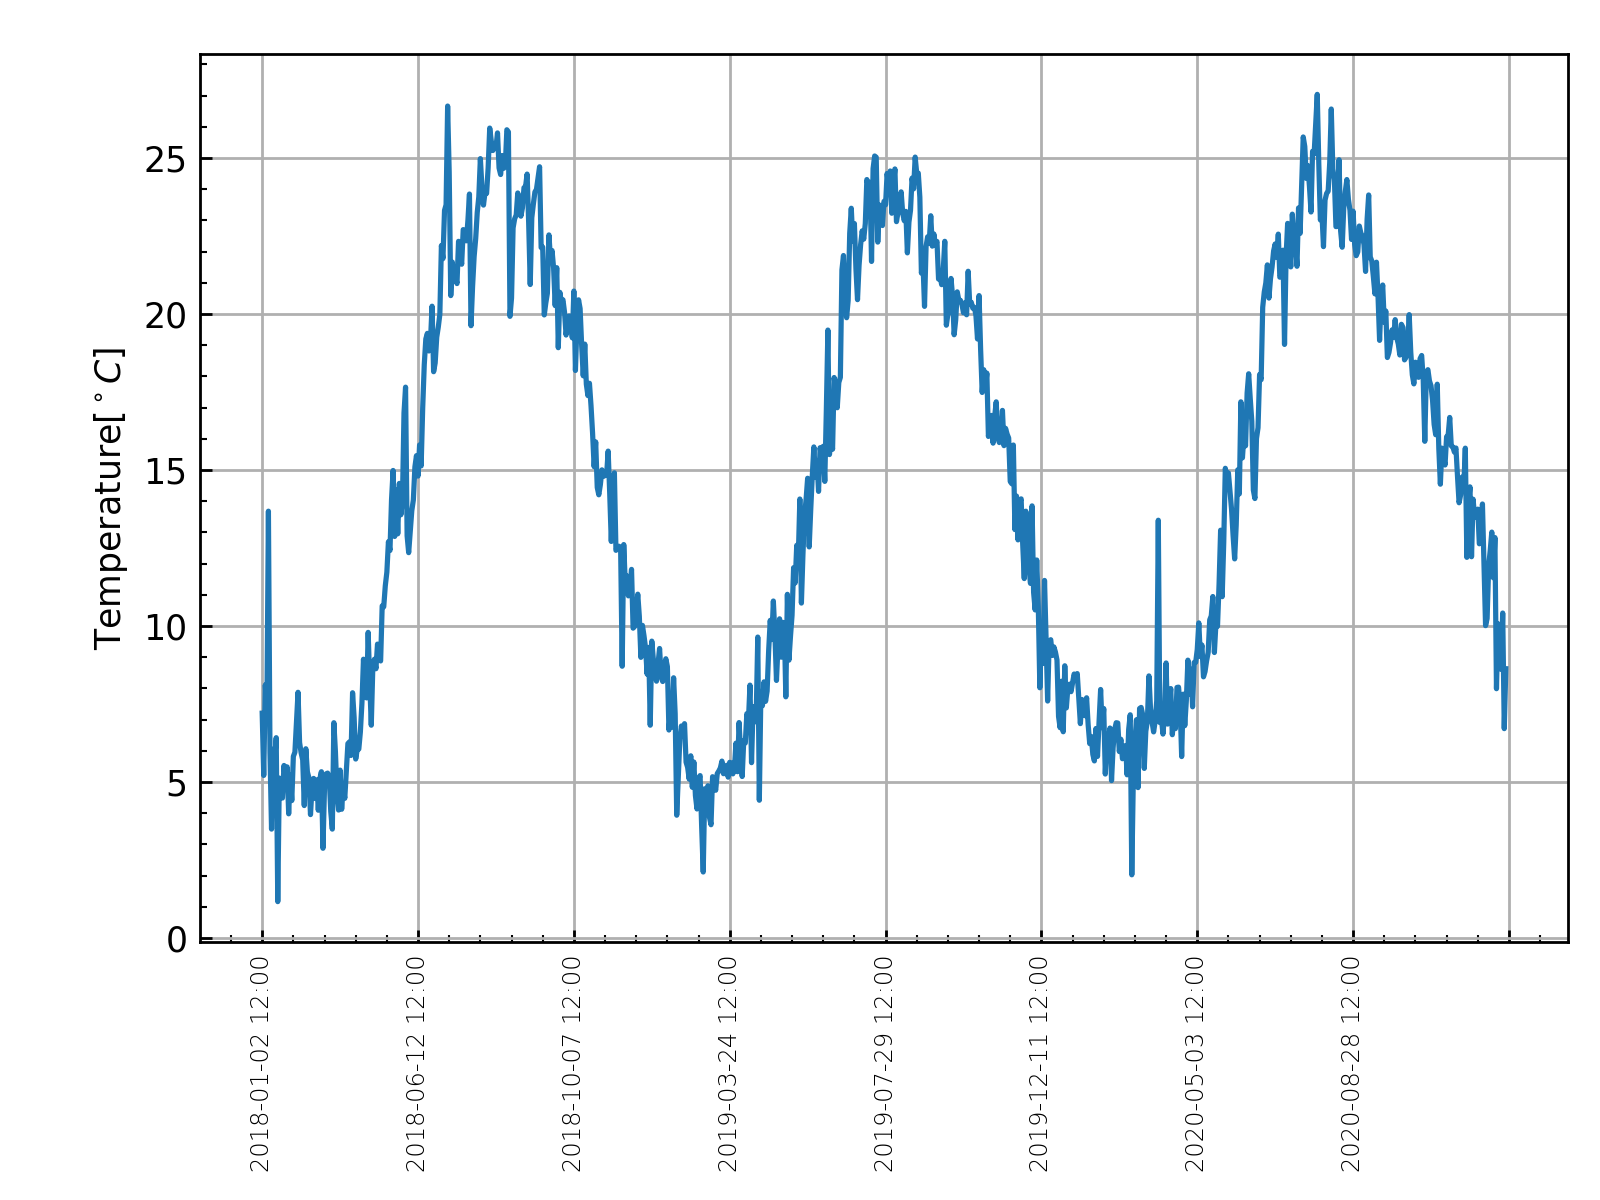
\includegraphics[scale=0.5]{figs/plots/sst.png}}
    \quad
    \subfloat[Chlorophyll-A($mg/m^3$)]{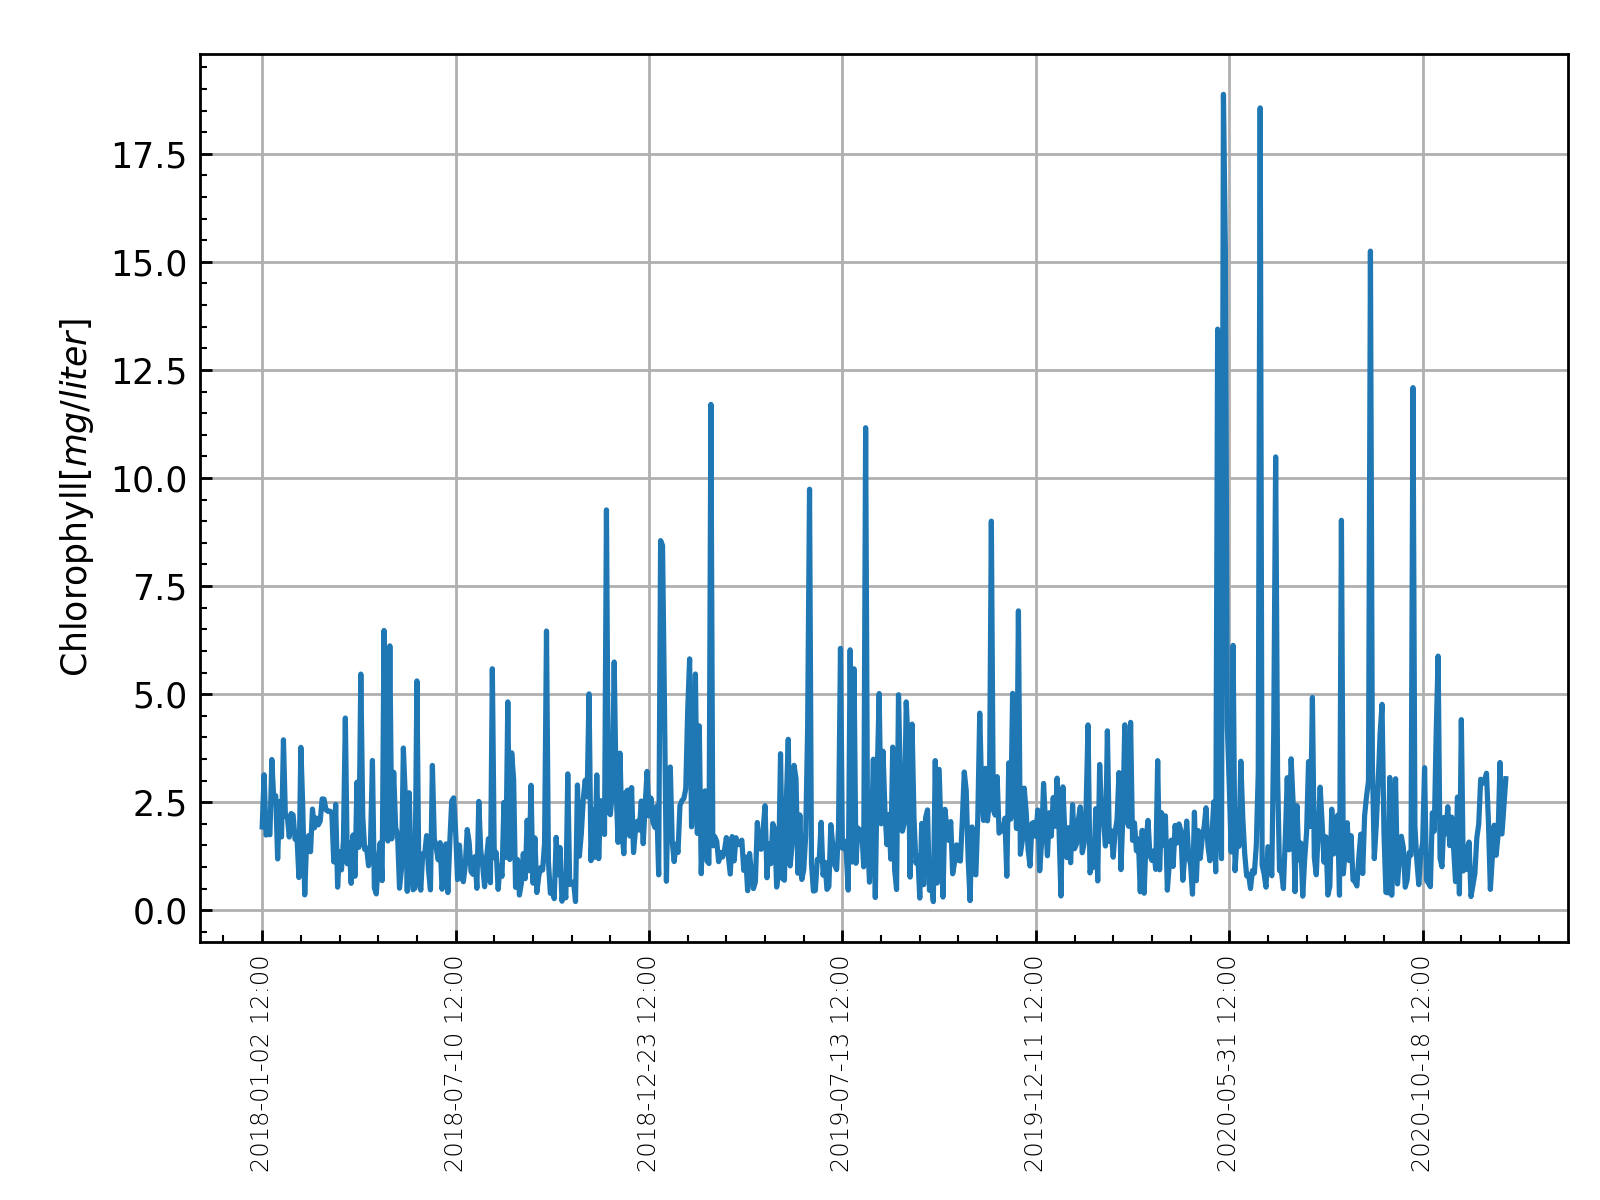
\includegraphics[scale=0.5]{figs/plots/chlor_a.png}}
    \label{fig:aqua_sst}
    \caption{AQUA-MODIS}
\end{figure}

\subsection{Verification}
    By plotting a correlation matrix between the field sea temperature and MODIS sea surface temperature we can make sure they are consistent with each other thus reduceing the possibility of an error.    
we verify our correlation of in-situ measured temperature and remotely observed SST.

\begin{figure}[H]
    \centering
    \subfloat[In-situ sea temperature vs MODIS SST]{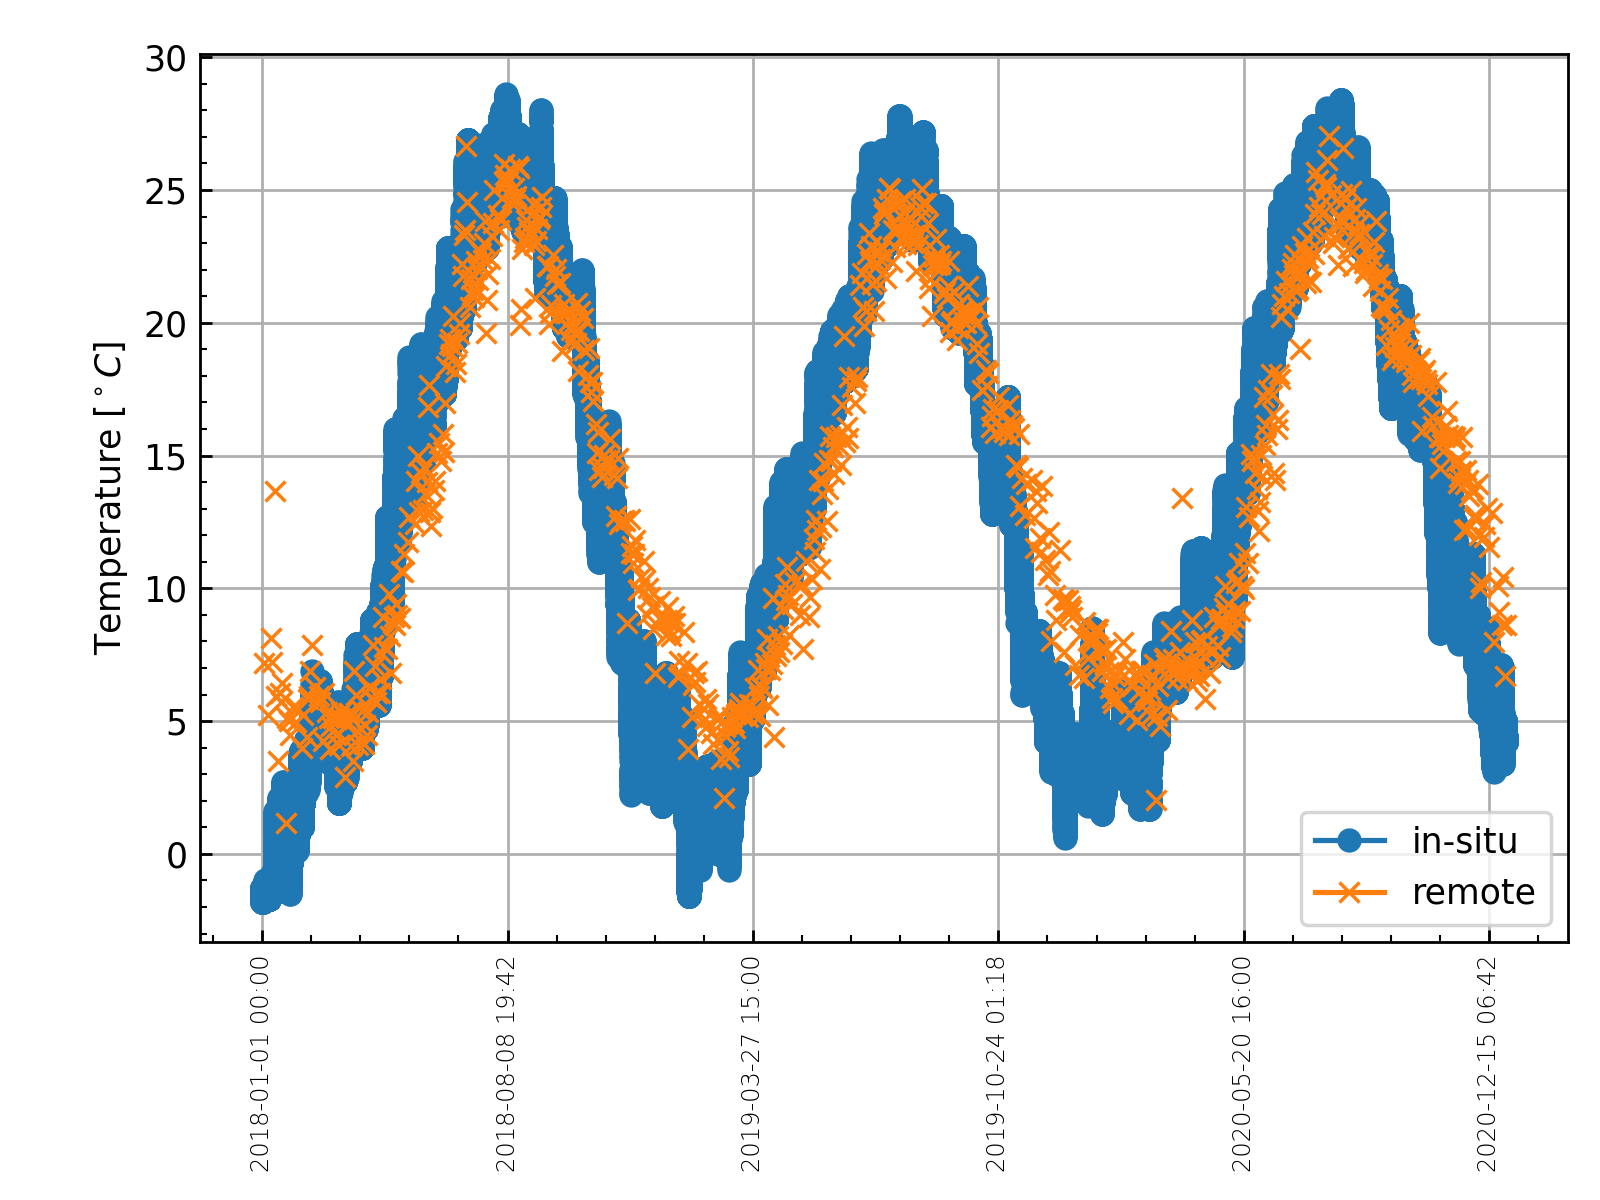
\includegraphics[scale=0.55]{figs/plots/temp_vs_sst.png}}
    \quad
    \subfloat[Correlation matrix]{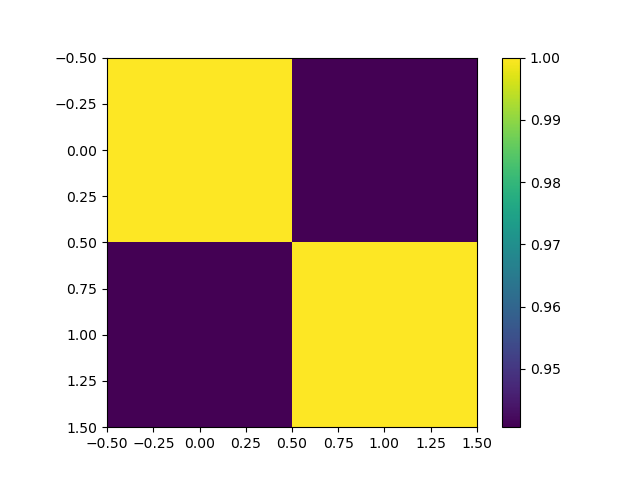
\includegraphics[scale=0.4]{figs/plots/temp_vs_sst_corr.png}}
    \caption{Verification of in-situ temperature and AQUA-MODIS SST($11\mu m$)}
\end{figure}

\begin{figure}[H]
    \centering
    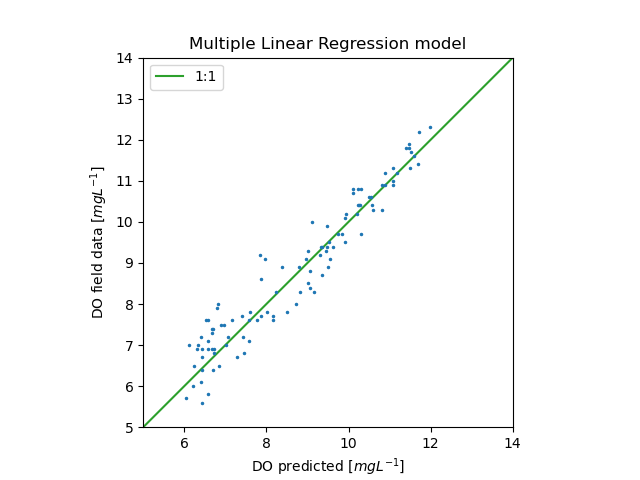
\includegraphics[scale=1.0]{figs/plots/mlr_test.png}
    \caption{Model test}
\end{figure}

Fig.17 suggests a good correlation with predictions and test labels of the data. We find that there is 24\% error associated with our predictions which could be reduced by using more longer and vivid datasets.